\documentclass[12pt]{article}

\usepackage{geometry}
  \geometry{
    a4paper,
    total={6in, 9in},
    top=20mm,
  }

\usepackage{graphicx}
\graphicspath{ {./img/} }

\usepackage{array}
\newcolumntype{P}[1]{>{\centering\arraybackslash}p{#1}}

\usepackage{multirow}
\usepackage{subcaption}
\usepackage{hyperref}

\usepackage{pgfplots}
\pgfplotsset{width=5in,compat=1.9}

\title{Homework 1}
\author{Stamate Valentin 2B4}

\begin{document}

\maketitle

\section*{Abstract}

While the problems became more complex, finding an efficient algorithm to solve that problem became harder.
This is why heuristic algorithms were a good alternative. The results given are pretty close and they have a better time complexity.

\section{Introduction}

The raport contain contain the results, comparisons and a conclusion of my algorithms. The problem is finding the global minimum of a function with various dimensions.
The motivation is to see if the methods I used(hich will be discussed in the next section) gives a good result for small or big imputs.
To test the algorithms I selectd 4 functions: \href{http://www.geatbx.com/docu/fcnindex-01.html#P89_3085}{\textbf{DeJong's function}}, \href{http://www.geatbx.com/docu/fcnindex-01.html#P150_6749}{\textbf{Schwefel's function}},
\href{http://www.geatbx.com/docu/fcnindex-01.html#P140_6155}{\textbf{Rastrigin's function}} and \href{http://www.geatbx.com/docu/fcnindex-01.html#P204_10395}{\textbf{Michalewicz's function}}. As you can see each one has a
different number of local minimum points.


\begin{center}
  \begin{figure}
  
    \begin{subfigure}{0.5\textwidth}
    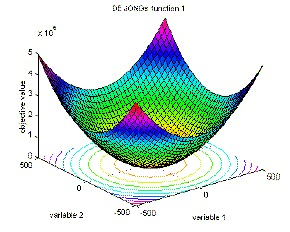
\includegraphics[width=0.9\linewidth, height=5cm]{dejong.jpg} 
    \caption{DeJong's function}
    \label{fig:subim1}
    \end{subfigure}
    \begin{subfigure}{0.5\textwidth}
    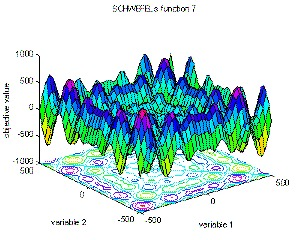
\includegraphics[width=0.9\linewidth, height=5cm]{schwefel.jpg}
    \caption{Schwefel's function}
    \label{fig:subim2}
    \end{subfigure}
    
  \end{figure}
  
  \begin{figure}
  
    \begin{subfigure}{0.5\textwidth}
    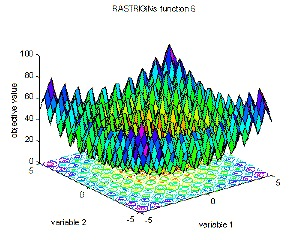
\includegraphics[width=0.9\linewidth, height=5cm]{rastrigin.jpg} 
    \caption{Rastrigin's function}
    \label{fig:subim3}
    \end{subfigure}
    \begin{subfigure}{0.5\textwidth}
    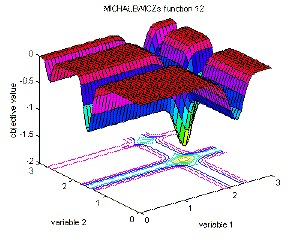
\includegraphics[width=0.9\linewidth, height=5cm]{michalenwicz.jpg}
    \caption{Michalewicz's function}
    \label{fig:subim2}
    \end{subfigure}
    
  \end{figure}
  
\end{center}






\section{Methods}
 
I used three methods: \href{https://en.wikipedia.org/wiki/Hill_climbing}{\textbf{HillClimbing - First Improvement}}, \href{https://en.wikipedia.org/wiki/Hill_climbing}{\textbf{HillClimbing - Best Improvement}} and 
\href{ttps://en.wikipedia.org/wiki/Simulated_annealing}{\textbf{Simulated Annealing}} for each function. I combined HCFI and HCBI by adding a simple condition after finding the first neighbour.

For representing the numbers I used a bit map that contain all components of a point. This way I can easily generate a random neighbour. In my algorithm one neighbour in HC is one that has the most unsignificant bit changed
the same way in numbers I add and subtract 1, but manipulating the bits. To generate a neighbour in SA I only negate one bit from the bit map. The main difference between SA and HC is that in SA I can choose a bad neighbour with a small probability.
This was SA has a larger domain exploration than HC.

The initialization is the same for all methods. I generate a bit map with 0 or 1 for each position. 

The HCFI algorithm stops when it cannot find any better neighbours. SA algorithm stops when is reaching a temperature eqal with \( 10^-8 \).


\section{Experiment Description}
Each method I combined it with it's iterated version. The number of repetitions are equal with \( 10^5 \), enought to get a good result. To see how the methods are behaving over different inputs I choose 2, 5, 10, 15 and 30 as point dimension. The precision for each component is 5 meaning \( \epsilon = 10^-5 \).
And the number global repetition is 30.


\section{Results}
Below are the results, a table for every input. Every cell has multiple values in this order: minimum value returned, running time, mean and standard distribution.

\begin{center}
  \begin{tabular}{ |P{2cm}||P{4cm}|P{4cm}|P{4cm}|  }
      
    \hline
    \multicolumn{4}{|c|}{ Algorithm Result (2) } \\
    
    \hline
      function & HCFI & HCBI & SA \\
    \hline

    De Jong     & \( 1.81899e^-10 \) & \( 1.81899e^-10 \) & \( 4.73165e^-10 \) \\
                & 17s & 19s & 9s \\
                & \( 1.81899e^-10 \) & \( 1.81899e^-10 \) &  \( 8.665234e^-6 \) \\
                & \( 0 \) & \( 0 \) & \( 2.359996e^-5 \) \\
    \hline
    Schwefel    & \( -837.964 \) & \( -837.964 \) & \( -837.966 \) \\
                & 27s & 30s & 12s \\
                & \( -837.9059 \) & \( -837.903 \) &  \( -837.8847 \) \\
                & \( 0.04788257 \) & \( 0.05601569 \) & \( 0.08802122 \) \\
    \hline
    Rastrigin   & \( 1.80426e-08 \) & \( 1.80426e-08 \) & \( 0 \) \\
                & 21s & 23s & 9s \\
                & \( 1.80426e-08 \) & \( 1.80426e-08 \) &  \( 0.005112576 \) \\
                & \( 0 \) & \( 0 \) & \( 0.007384009 \) \\
    \hline
    Michalewicz & \(-0.801323\) & \(-0.801323\) & \(-0.801323\) \\
                & 22s & 23s & 9s \\
                & \( -0.8013227 \) & \( -0.8013223 \) &  \( -0.8013221 \) \\
                & \( 4.794633e-07 \) & \( -0.8013223 \) & \( 2.537081e-07 \) \\

    \hline
  \end{tabular}
\end{center}

\begin{center}
  \begin{tabular}{ |P{2cm}||P{4cm}|P{4cm}|P{4cm}|  }
      
    \hline
    \multicolumn{4}{|c|}{ Algorithm Result (5) } \\
    
    \hline
      function & HCFI & HCBI & SA \\
    \hline

    De Jong     & \( 4.54747e-10 \) & \( 4.54747e-10 \) & \( 2.23713e-07 \) \\
                & 1m 56s & 1m 37s & 24s \\
                & \( 4.54747e-10 \) & \( 4.54747e-10 \) &  \( 0.04696127 \) \\
                & \( 0 \) & \( 0 \) & \( 0.1665665 \) \\
                \hline
    Schwefel    & \( -2088.19 \) & \( -2057.46 \) & \( -2053.71 \) \\
                & 3m 12s & 2m 54s & 37s \\
                & \( -1991.65 \) & \( -1995.07 \) &  \( -1895.261 \) \\
                & \( 46.19519 \) & \( 38.03182 \) & \( 79.70068 \) \\
                \hline
    Rastrigin   & \( 1.80426e-08 \) & \( 1.80426e-08 \) & \( 5.95225 \) \\
                & 2m 44s & 2m 18s & 28s \\
                & \( 1.80426e-08 \) & \( 1.80426e-08 \) &  \( 9.125848 \) \\
                & \( 0 \) & \( 0 \) & \( 2.059847 \) \\
                \hline
    Michalewicz & \( -3.69195 \) & \( -3.68325 \) & \( -3.6938 \) \\
                & 3m 13s & 2m 55s & 30s \\
                & \( -3.656661 \) & \( -3.646231 \) &  \( -3.460571 \) \\
                & \( 0.02152056 \) & \( 0.01848281 \) & \( 0.131784 \) \\

    \hline
  \end{tabular}
\end{center}

\begin{center}
  \begin{tabular}{ |P{2cm}||P{4cm}|P{4cm}|P{4cm}| }
      
    \hline
    \multicolumn{4}{|c|}{ Algorithm Result (10) } \\
    
    \hline
      function & HCFI & HCBI & SA \\
    \hline

    De Jong     & \(9.09495e^-10\) & \( 9.09495e^-10 \) & \( 1.05876e^-6 \) \\
                & 14m &  8m & 59s \\
                & \( 9.09495e^-10 \) & \( 9.09495e^-10 \) &  \( 0.0001858588 \) \\
                & \( 0 \) & \( 0 \) & \( 0.0004888328 \) \\
                \hline
    Schwefel    & \( -3634.03 \) & \( -3742.84 \) & \( -3630.58 \) \\
                & 23m & 11m & 59s \\
                & \( -3394.599 \) & \( -3440.418 \) &  \( -3211.317 \) \\
                & \( 97.74172 \) & \( 115.7556 \) & \( 247.4637 \) \\
                \hline
    Rastrigin   & \( 1.80426e^-8 \) & \( 1.80426e^-8 \) & \( 8.68414 \) \\
                & 18m & 9m & 53s \\
                & \( 1.80426e^-8 \) & \( 1.80426e^-8 \) &  \( 25.81046 \) \\
                & \( 0 \) & \( 0 \) & \( 9.338441 \) \\
                \hline
    Michalewicz & \( -7.84583 \) & \( -7.60421 \) & \( -8.1224 \) \\
                & 19m &  10m & 45s \\
                & \( -7.05834 \) & \( -7.131895 \) &  \( -6.258278 \) \\
                & \( 0.2676364 \) & \( 0.2289028 \) & \( 1.08582 \) \\

    \hline
  \end{tabular}
\end{center}

\begin{center}
  \begin{tabular}{ |P{2cm}||P{4cm}|P{4cm}|P{4cm}| }
      
    \hline
    \multicolumn{4}{|c|}{ Algorithm Result (15) } \\
    
    \hline
      function & HCFI & HCBI & SA \\
    \hline

    De Jong     & \( 1.36424e^-9 \) & \( 1.36424e^-9 \) & \( 1.29213e^-6 \) \\
                & 40m & 17m & 1m 25s \\
                & \( 1.36424e^-9 \) & \( 1.36424e^-9 \) &  \( 0.3072009 \) \\
                & \( 0 \) & \( 0 \) & \( 1.222033 \) \\
                \hline
    Schwefel    & \( -4996.19 \) & \( -4932.18 \) & \( -5035.86 \) \\
                & 1h 4m & 25m & 1m 31s \\
                & \( -4675.259 \) & \( -4646.454 \) &  \( -4216.178 \) \\
                & \( 143.6435 \) & \( 131.4299 \) & \( 479.3601 \) \\
                \hline
    Rastrigin   & \( 1.80426e^-8 \) & \( 1.80426e^-8 \) & \( 20.3447 \) \\
                & 51m & 21m & 1m 18s \\
                & \( 1.80426e^-8 \) & \( 1.80426e^-8 \) &  \( 36.68338 \) \\
                & \( 0 \) & \( 0 \) & \( 10.20887 \) \\
                \hline
    Michalewicz & \( -10.938 \) & \( -10.6536 \) & \( -11.9283 \) \\
                & 44m & 20m & 1m 6s \\
                & \( -9.793424 \) & \( -9.765478 \) &  \( -8.65901 \) \\
                & \( 0.3922462 \) & \( 0.2919562 \) & \( 2.086646 \) \\

    \hline
  \end{tabular}
\end{center}

\begin{center}
  \begin{tabular}{ |P{2cm}||P{4cm}|P{4cm}|P{4cm}| }
      
    \hline
    \multicolumn{4}{|c|}{ Algorithm Result (30) } \\
    
    \hline
      function & HCFI & HCBI & SA \\
    \hline

    De Jong     & \( 2.72848e^-09 \) & \( 2.72848e^-9 \) & \( 0.0883307 \) \\
                & 5h 48m & 1h 11m & 2m 56s \\
                & \( 2.72848e^-9 \) & \( 2.72848e^-9 \) &  \( 2.972082 \) \\
                & \( 0 \) & \( 0 \) & \( 2.592697 \) \\
                \hline
    Schwefel    & \( -8481.25 \) & \( -8437.5 \) & \( -10557.7 \) \\
                & 8h 43m & 1h 36m & 2m 57s \\
                & \( -8062.989 \) & \( -8069.389 \) &  \( -9186.45 \) \\
                & \( 145.3006  \) & \( 164.2671 \) & \( 601.2258 \) \\
                \hline
    Rastrigin   & \( 1.80426e^-8 \) & \( 1.80426e^-8 \) & \( 57.882 \) \\
                & 7h 11m & 1h 25m & 2m 40s \\
                & \( 1.80426e^-8 \) & \( 1.80426e^-8 \) &  \( 93.20304 \) \\
                & \( 0 \) & \( 0 \) & \( 19.97291 \) \\
                \hline
    Michalewicz & \( -17.7899 \) & \( -17.5032 \) & \( -23.5971 \) \\
                & 7h 40m & 1h 37m & 2m 18s \\
                & \( -16.48712 \) & \( -16.40962 \) &  \( -20.7609 \) \\
                & \( 0.5326 \) & \( 0.3950859 \) & \( 1.685605 \) \\

    \hline
  \end{tabular}
\end{center}


This graph represents the evolution of time when increasing the input size. The input is the number of components the function receives. I choose the Rastrigin's function because it has many local minimum points.


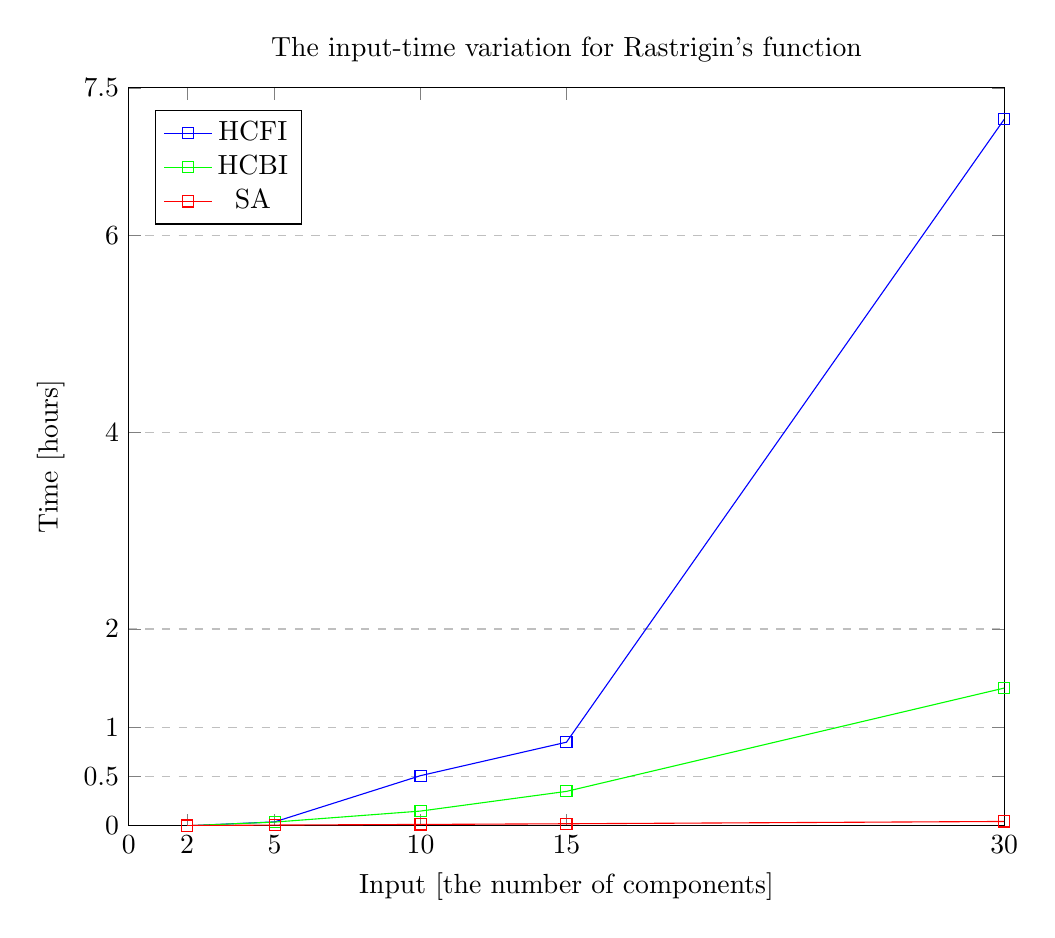
\begin{tikzpicture}
  \begin{axis}[
      title={The input-time variation for Rastrigin's function},
      xlabel={Input [the number of components]},
      ylabel={Time [hours]},
      xmin=0, xmax=30,
      ymin=0, ymax=7.5,
      xtick={0,2, 5,10,15,30},
      ytick={0,0.5,1,2,4,6,7.5},
      legend pos=north west,
      ymajorgrids=true,
      grid style=dashed,
  ]
  
  \addplot[
      color=blue,
      mark=square,
      ]
      coordinates {
      (2, 0.0005)(5, 0.04)(10, 0.51)(15, 0.85)(30, 7.18)
      };
      \addlegendentry{HCFI}
      
  \addplot[
      color=green,
      mark=square,
      ]
      coordinates {
      (2, 0.0006)(5, 0.038)(10, 0.15)(15, 0.35)(30, 1.4)
      };
      \addlegendentry{HCBI}

  \addplot[
      color=red,
      mark=square,
      ]
      coordinates {
      (2, 0.0025)(5, 0.0077)(10, 0.014)(15, 0.021)(30, 0.0444)
      };
      \addlegendentry{SA}
      
  \end{axis}
\end{tikzpicture}


So, as shown in this graph the input has a signifficant time impact for HC algorithms. SA time doesn't change that much. 


\section{Comparisons}
Next, I will discuss about the differences between these algorithms. The HC algorithm pick always a good neighbour: the best or the first. On the other side, SA algorithms
can choose a bad neighbour but this chance descreases together with temperature. This way SA algorithm can explore more while HC algorithm can ramain stuck in a local minimum.
Also, can be seen that SA algorithm is much more time efficient while giving a good result. But, increasing the input size, SA algorithm gives a more general result than a close one.
Between the two HC methods, best improvement seems to be better and have a better time.

\section{Conclusions}
Finding global minimum can be a challenging goal. Deterministic algorithms can find it with backtracking but the time complexity makes it impossible to run in real time with big inputs.
So, I tested three heuristic algorithms Hill Climbing first and best improvement and Simulated Annealing. 

  
   My conclusion is that SA can be a very good candidate for use cases bacause it is very fast comparing with
HC algorithms witch gives a better result but they are much slower. 


\begin{thebibliography}{9}
  \bibitem{}
    \url{https://stackoverflow.com/questions/26282709/heuristic-algorithm-for-finding-minimal-value-from-function/26283364}
  \bibitem{}
    \url{https://en.wikipedia.org/wiki/Hill_climbing}
  \bibitem{}
    \url{https://en.wikipedia.org/wiki/Simulated_annealing}
  \bibitem{}
    \url{https://www.youtube.com/watch?v=S9vs05eAGN0&ab_channel=EricSchirtzinger}
  \bibitem{}
    Second seminar notes
  \bibitem{}
    \url{http://www.geatbx.com/docu/fcnindex-01.html#P89_3085}
  \bibitem{}
    \url{http://www.geatbx.com/docu/fcnindex-01.html#P150_6749}
  \bibitem{}
    \url{http://www.geatbx.com/docu/fcnindex-01.html#P140_6155}
  \bibitem{}
    \url{http://www.geatbx.com/docu/fcnindex-01.html#P204_10395}
  \bibitem{}
    \url{https://www.geeksforgeeks.org/function-pointer-in-c/}
  \bibitem{}
    \url{https://stackoverflow.com/questions/59565481/create-a-vector-from-a-txt-data-file-in-r}
  \end{thebibliography}  
  


\end{document}